
\documentclass[12pt, a4paper]{article}
\usepackage{ragged2e}
\usepackage[margin=1in]{geometry}
\usepackage[utf8]{inputenc}
%\usepackage[tablesfirst,nolists]{endfloat}
\usepackage[toc,page]{appendix}
\usepackage{times}
\usepackage[flushleft]{threeparttable}
\usepackage{hyperref}
\usepackage{authblk}
\usepackage{setspace}
\usepackage{apacite}
\usepackage{caption}
\usepackage{graphicx}
\usepackage{titlesec}
\usepackage{color}
\usepackage{endnotes}
\usepackage{caption}
\usepackage{textcase}
\usepackage{booktabs}
\usepackage{titling}
\usepackage{authblk}

\renewcommand\appendixpagename{Appendix}

\captionsetup{
  labelsep=newline,
  justification=raggedright,
  singlelinecheck=false
}

\pagestyle{myheadings}
\title{}
\author{}
\date{}
\doublespacing
%\renewcommand{\efloatheading}[1]{}

\renewcommand{\appendixname}{Appendix}
\titleformat{name=\section,numberless}[hang]
   {\bfseries}{}{6pt}{\Large}


%\let\footnote=\endnote


\begin{document}

\title{A zero attraction effect in naturalistic choice}

\author{Anna Trendl$^{a,*}$ \\ \href{mailto:a.trendl@warwick.ac.uk}{a.trendl@warwick.ac.uk}\\
 \and Neil Stewart$^b$ \\ 
 \href{mailto:neil.stewart@wbs.ac.uk}{neil.stewart@wbs.ac.uk}
 \\ 
 \and Timothy L. Mullett$^b$ \\
 \href{mailto:Tim.Mullett@wbs.ac.uk}{Tim.Mullett@wbs.ac.uk}
 \\}
 
\date{
    $^a$Department of Psychology, University of Warwick, University Road, Coventry, CV4 7AL, United Kingdom\\
    $^b$Warwick Business School, University of Warwick, Scarman Road, Coventry, CV4 7AL, UK\\
    $^*$Corresponding author\\[2ex]%
    \today
}



\begin{titlepage}
%\maketitle
\thispagestyle{empty}
\maketitle
\centering
    This research was funded in part by Economic and Social Research Council grants ES/K002201/1, ES/P008976/1, and ES/N018192/1, and Leverhulme Trust grant RP2012-V-022. 
\clearpage
\thispagestyle{empty}
\RaggedRight
\begin{center}
\LARGE{A zero attraction effect in naturalistic choice}
\end{center}
\begin{abstract}
\noindent
In the attraction effect, adding a dominated third option to a choice set of two options can reverse the preference for the original two options, and even increase one of the option's choice share. This constitutes a violation of the axioms of regularity and independence from irrelevant alternatives, which are core properties of any choice model in which the utility of each option is stable across choice sets. In the past 20 years, the attraction effect has driven the development of a set of influential models of multiattribute choice. However, two studies (\citeNP{Frederick2014} and \citeNP{Yang2014}) involving a large number of experiments with naturalistic choice options (e.g., snacks, movies) found no evidence for the attraction effect in choice contexts where options have no numerical attribute dimensions -- a finding which would severely undermine its theoretical importance. \citeA{Huber2014} criticised these experiments, laying down a set of criteria that should be met by any experiment wishing to test for the attraction effect in real-world consumer choices. Based on these criteria, this article presents a carefully designed experiment testing the attraction effect with movies as naturalistic choice options. The results show a precisely zero attraction effect.
%172 words now
\end{abstract}


\end{titlepage}



\newpage
\RaggedRight

\section*{The attraction effect}


Imagine that you are having a nice meal in a restaurant, and you are looking at the two dessert options available on the menu: cheesecake and pecan pie. You are torn between the creamy texture of the cheesecake, and the rich, nutty flavour of the pecan pie. You resolve to have the cheesecake. As the waiter approaches to take your order, he informs you that a third dessert option, apple pie---which you find quite bland---is also available today. But now you have changed your mind, and decide to order the pecan pie. \citeA{Tsetsos2010} give just this paradoxical example: the availability of the apple pie, which you do not want, makes you switch from cheesecake to pecan pie.

This is an example of the attraction effect (also known as asymmetric dominance effect). The presence of the apple pie (decoy) in the choice set makes you more likely to choose the pecan pie (target) over the cheesecake (competitor). In essence, it states that when the decision maker is indifferent between the target and the competitor (pecan pie and cheesecake in the example), the addition of an inferior decoy option that resembles the target (apple pie is similar to pecan pie, but is less liked by the decision maker) increases the likelihood that the target will be chosen.


The attraction effect is important, because it poses a challenge to all choice models that rely on the assumption that preferences can be represented on a cardinal utility scale. This assumption is called simple scalability, and is one of the consequences of Luce's choice axiom \cite{Luce1959}. Crucially, the attraction effect represents a violation of independence of irrelevant alternatives, which requires that the preference ranking of two options should not be affected by adding new options to the choice set. In addition, the attraction effect violates the axiom of regularity, which states that an option's choice probability cannot increase when the choice set is extended (\citeNP{Luce1977a}; \citeNP{Tversky1972a}). Therefore, the existence of the attraction effect implies that the utility of a choice option cannot be represented by a single internal magnitude that is invariant to the other options in the choice set.

Owing to its theoretical importance, the attraction effect has played a substantial role in the evolution of multialternative, multiattribute models of choice, with a significant number of various theoretical accounts being developed over the past 20 years (e.g., multialternative decision field theory, \citeNP{Roe2001a}; leaky competing accumulators, \citeNP{Usher2004b}; multialternative attentional drift-diffusion model,   \citeNP{Krajbich2010a}; range-normalization model, \citeNP{Soltani2012}; associative accumulation model, \citeNP{Bhatia2013b}; multiattribute linear ballistic accumulator, \citeNP{Trueblood2014a}; multialternative decision by sampling, \citeNP{Noguchi2018a}).



The first multiattribute choice experiments demonstrating the attraction effect (e.g., \citeNP{Huber1982}; \citeNP{Simonson1992}) almost exclusively used stimuli presented as a set of numerical attributes (e.g., cars presented as numerical values for gas mileage and ride quality). \citeA{Trueblood2013a} have also found evidence for the attraction effect in a perceptual choice experiment, where participants were asked to select the largest from three rectangles with varying widths and heights. 


However, recent research suggests that the attraction effect might only occur under very specific conditions.
In particular, it had been shown that the effect is much more likely to occur when an attribute-wise comparison strategy is employed in the choice process as opposed to an alternative-wise strategy \cite{Noguchi2014a}. One implication of the importance of the underlying comparison strategy is that the strength of the attraction effect seems to be highly dependent on the exact presentation format of the numerical or perceptual choice options (e.g., \citeNP{Spektor2018}; \citeNP{Cataldo2019}). A natural concern is then whether this hugely influential decision bias generalises to real-world choice situations, where attributes often cannot be easily visually represented and compared.  


While choice options with binary attribute dimensions (perceptual or numerical) can be easily manipulated within a choice experiment, most real-world choices involve complex, naturalistic objects with a large number of underlying attributes. Recent experiments in multiattribute choice introduced what can perhaps be considered as more ecologically valid stimuli (e.g., movies presented as thumbnails and titles on Netflix, or photographs of popular snacks). Results from these experiments indicate that there might be significant differences in the processing of numerical and naturalistic stimuli. For example, \citeA{Bhatia2018b} find that, with naturalistic stimuli, the weighted additive model on a high-dimensional semantic representation generalises to new choices better than the simpler heuristic models, which perform so well on stimuli presented as sets of numerical attributes.

Recently, the existence of the attraction effect in choices that involve naturalistic options has become a contentious issue in the decision-making literature. Based on 38 experiments, \citeA{Frederick2014} presented an extensive investigation of the boundary conditions of the attraction effect. These experiments included choice options with numerical attributes, as well as complex, real-world stimuli (e.g., fruits, bottled water, apartments, etc.), and in some of these experiments, participants could even sample the choice options (e.g. Kool-Aid, facial tissue, jelly beans). The overall conclusion of this study was that while the presence of the decoy seemed to affect choices when the options had numerical attributes, it was absent in experiments with more complex, naturalistic stimuli. In light of these results, \citeauthor{Frederick2014} posited that the psychological processes underlying decisions that involve options with numeric attributes are fundamentally different from those employed in decisions where the stimuli has a more naturalistic format. This conclusion was also supported by \citeA{Yang2014}, who reported difficulties replicating the attraction effect in experiments where the stimuli were pictorial, as opposed to cases where the attributes were presented numerically.

These two studies sparked considerable interest amongst decision making researchers, and led to the re-examination of the boundary conditions of the attraction effect. While the results from these studies are consistent in showing no evidence for the attraction effect across a wide variety of naturalistic choice options, the degree to which the individual experiments presented in these studies invoked an attraction effect-type choice scenario, and thus constitute a stringent test of the attraction effect has been subsequently questioned.
  
In particular, \citeA{Huber2014} discussed five critical conditions that can inhibit the attraction effect, and argued that many of these are present in the experiments reported by \citeA{Frederick2014} and \citeA{Yang2014}. The five critical conditions are to avoid: (1) strong prior preferences over the target and competitor, (2) inability to identify the dominance relationship  between the target and the decoy, (3) heterogeneity in prior preferences over the target and competitor, (4) an undesirable decoy and (5) a decoy that is too desirable. In addition, \citeA{Simonson2014a} further stressed the importance of the detection of the dominance relationship in observing the attraction effect. 


Due to the theoretical significance of the attraction effect, it is important to know if the attraction effect is confined to choice settings with stimuli presented in an attribute by alternative format. Arguably, while most consumer choices in the real world involve stimuli that are often presented in a rich naturalistic form \cite{Bhatia2018b}, development of formal models of choice have been almost exclusively reliant on results from experiments where the options have numerical attributes. Exploring how the strength of the effect depends on the presentation format of the choice alternatives also provides us with invaluable information about the cognitive process underlying the attraction effect. In this article, we describe a test of the attraction effect with complex, naturalistic choice options, using a carefully developed experimental methodology that addresses all of the critical conditions discussed by \citeA{Huber2014}. In line with the results reported by \citeA{Frederick2014} and \citeA{Yang2014}, we find no evidence for the attraction effect.


\section*{Testing the attraction effect with real-world stimuli}

The goal of this experiment was to test the attraction effect with naturalistic stimuli. We chose to use the most popular movies on IMDb as stimuli. Since movies are an integral part of Western culture, we can reasonably expect that most our participants will be sufficiently interested in the choice options. Furthermore, choosing between movies is a realistic, everyday task. In addition, the movie space is rich, and thus it allows us to create a wide range of unique choice triplets to test the attraction effect.

When the stimuli have numerical attributes, it is straightforward to construct choice triplets with a target, competitor and decoy. 
However, with naturalistic stimuli, this task is significantly more complicated. \citeA{Frederick2014}  have also used movie stimuli in two of their experiments: they chose pairs of movies that are part of the same series or are starring the same actor (but have distinctly different genres) to create target-decoy pairs. In these experiments, the identity role of each of the three movies (target, competitor, decoy) was always the same for all participants, and based upon population average ratings rather than individual ratings.




Our novel experimental design takes individual preferences into account when creating target-competitor-decoy triplets, and ensures that decision makers are indifferent between the target and competitor and are able to clearly identify the inferiority of the decoy. To increase the statistical power of our experiment, we used a within-subjects design. We presented participants with both A, B, A' and B, A, B' triplet pairs (where X' is the dominated option). The triplet pairs were created from ``quadruplets'' (each made up of two choice triplets), using two distinctly different target-decoy pairs. Figure \ref{fig:quadruplets} shows an example of two choice triplets created from one such quadruplet.


\begin{figure}
\centering
		 \caption{Two choice triplets used in the experiment.}
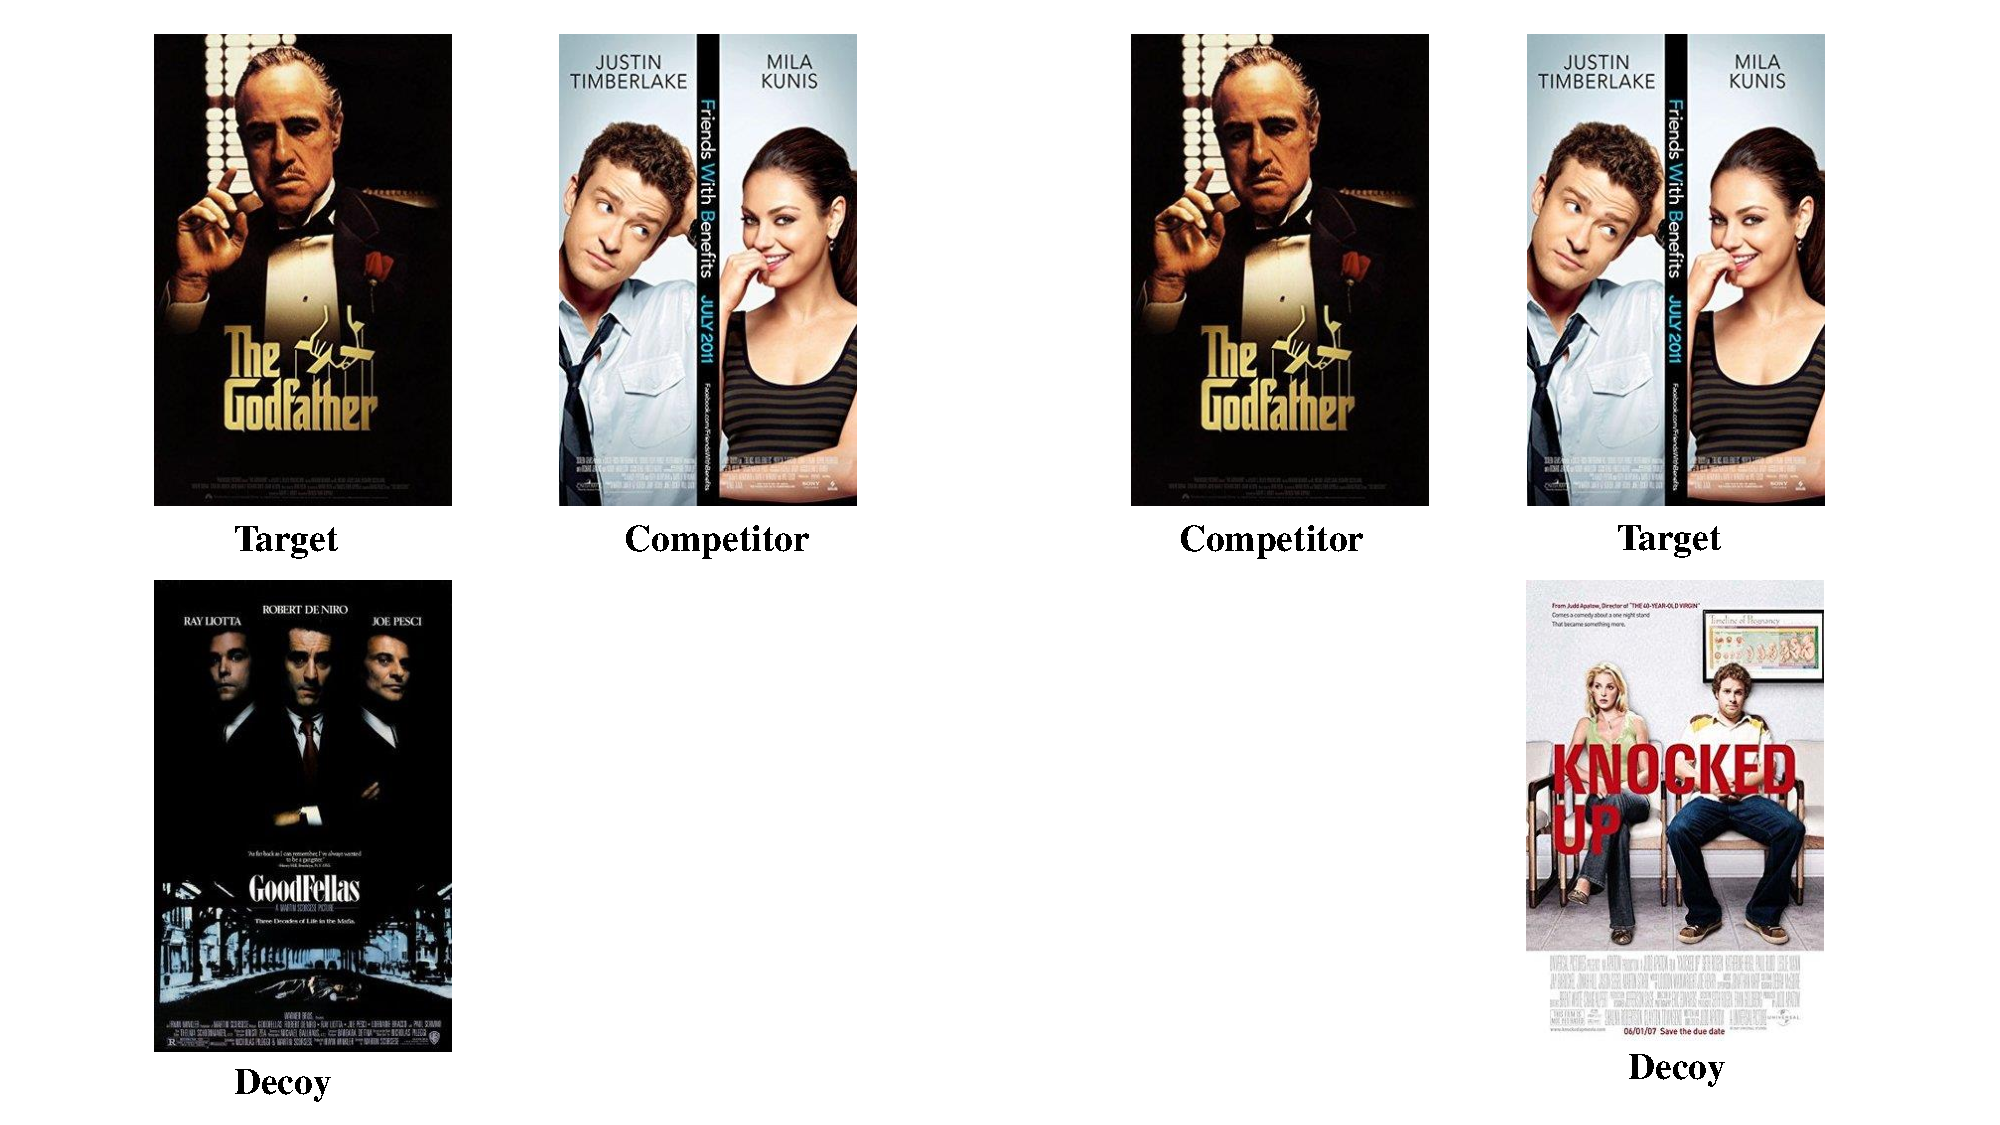
\includegraphics[width=1\textwidth]{figure1.pdf}
\label{fig:quadruplets}
\end{figure}

\subsection*{Method}

\subsubsection*{Preregistration.}
The study design, exclusion criteria and all the analyses were planned and registered before we collected any choice data. The pre-registration can be accessed \href{https://osf.io/fme6c/?view_only=31da4193689f4247a76af93b2f98fcef}{here}.

\subsubsection*{Candidate choice set selection.}

To determine the choice sets used in the experiment, the first step was to create a set of quadruplets, each consisting of two movies that are very similar (for the two target-decoy pairs; i.e., A--A', B--B'), whilst making sure that the two pairs are overall sufficiently different from each other (for the target-competitor pair; i.e., A--B).

The details of the construction of these quadruplets are somewhat arbitrary---a different recipe could have been used. However, the main point is that the choice triplets created from these quadruplets pass \citeauthor{Huber2014}'s \citeyear{Huber2014} criteria, as we detail below. The main steps in the quadruplet construction process we describe in detail in the remainder of this section are depicted in Figure \ref{fig:flow}.


To obtain the set of 400 movies, we first retrieved the most popular 40 movies from each of 10 distinct genre categories (romance, drama, sci-fi, thriller, comedy, horror, animation, fantasy, crime, action) from IMDb. The popularity of each movie was defined by the number of ratings it has received. We selected a wide range of genres to obtain a sufficiently rich stimuli space, as we wanted our participants to have a variety of preferences over our stimuli. We omitted any sequels.

Owing to the multidimensional nature of the stimuli, one of the main difficulties in creating attraction effect choice triplets from real-world objects is establishing a criterion for matching up similar objects. We used genre and sub-genre information from allmovie.com to create target-decoy pairs with many shared genres that are likely to be perceived as similar, and target-competitor pairs with no genre overlap that are likely to be perceived as different.

We conjectured that it will be harder to find movie pairs that will be perceived as similar, because any given movie is similar to a only a few movies, and dissimilar to all of the others. For this reason, we started the quadruplet creation with selecting potential target-decoy pairs.

\begin{figure}[htb!]
\centering
		\caption{Summary of the quadruplet construction process. }
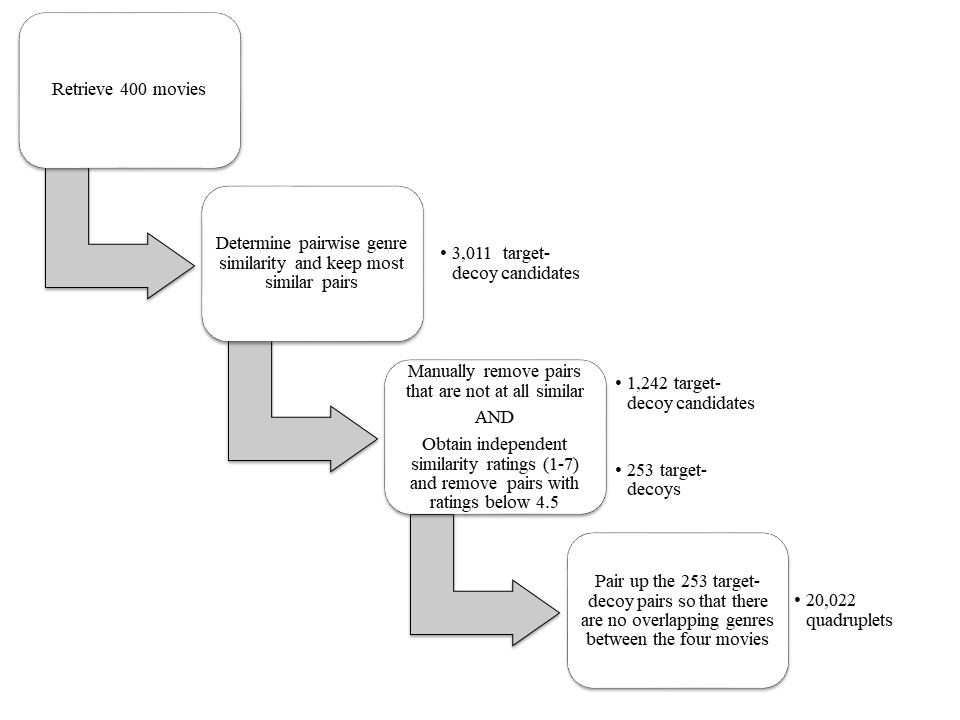
\includegraphics[width=0.9\textwidth]{flow.png}
\label{fig:flow}
\end{figure}

The genre information on allmovie.com is very rich: compared to the 18 genre categories on IMDb, there are 156 genre and sub-genre categories, capturing many important aspects of the movies. Using this rich genre information, we created a movie by movie ($400 \times 400$) matrix, where each cell was the number of overlapping genre categories between the two movies. We selected a movie pair as target-decoy candidate if, for a given target candidate movie, the number of overlapping genres with a candidate decoy was equal to the maximum overlap seen for that target across all candidate decoy movies. This resulted in 2,271 target-decoy candidate movie pairs overall.
We also added 806 movie pairs obtained from the mutually closest 10\% of movies based on a latent semantic analysis\footnote{The latent semantic analysis assesses the similarity of two items based on the text associated with them. For this analysis, we used the summary text about the movies as well as plot keywords, actor and director names, all retrieved from IMDb.} that were not already in our list of target-decoy candidates. The rationale behind using semantic proximity as an additional criterion was to capture movie pairs that are very close to each other in terms of the story themes, but are not the closest on the genre dimension. Overall, we had 3,011 unique target-decoy candidate pairs at this point.

We then reduced the size of this list by selecting the most similar movie pairs. This was done manually by two researchers, who independently judged the similarity of each movie pair (not similar at all/similar). We then only kept the movie pairs that were judged as similar by both researchers, weeding out the movie pairs that were obviously not similar, resulting in 1,242 target-decoy candidates. We then divided the 1,242 pairs into six groups of 207 pairs, and ran a pilot study where we asked 60 participants to rate the similarity of a randomly chosen group of movie pairs, obtaining 10 independent similarity ratings for each of the 1,242 target-decoy candidates. Participants rated the similarity of each movie pair on a 1--7 scale, which also included a ``don't know'' option. Figure \ref{fig:exp2_pilot}  shows the distribution of the average similarity ratings for each movie pair.

\begin{figure}[htb!]
\centering
		\caption{The distribution of the average similarity rating for each target-decoy candidate pair (N = 1242). The dotted line is the cut-off value for accepting a movie pair as similar}
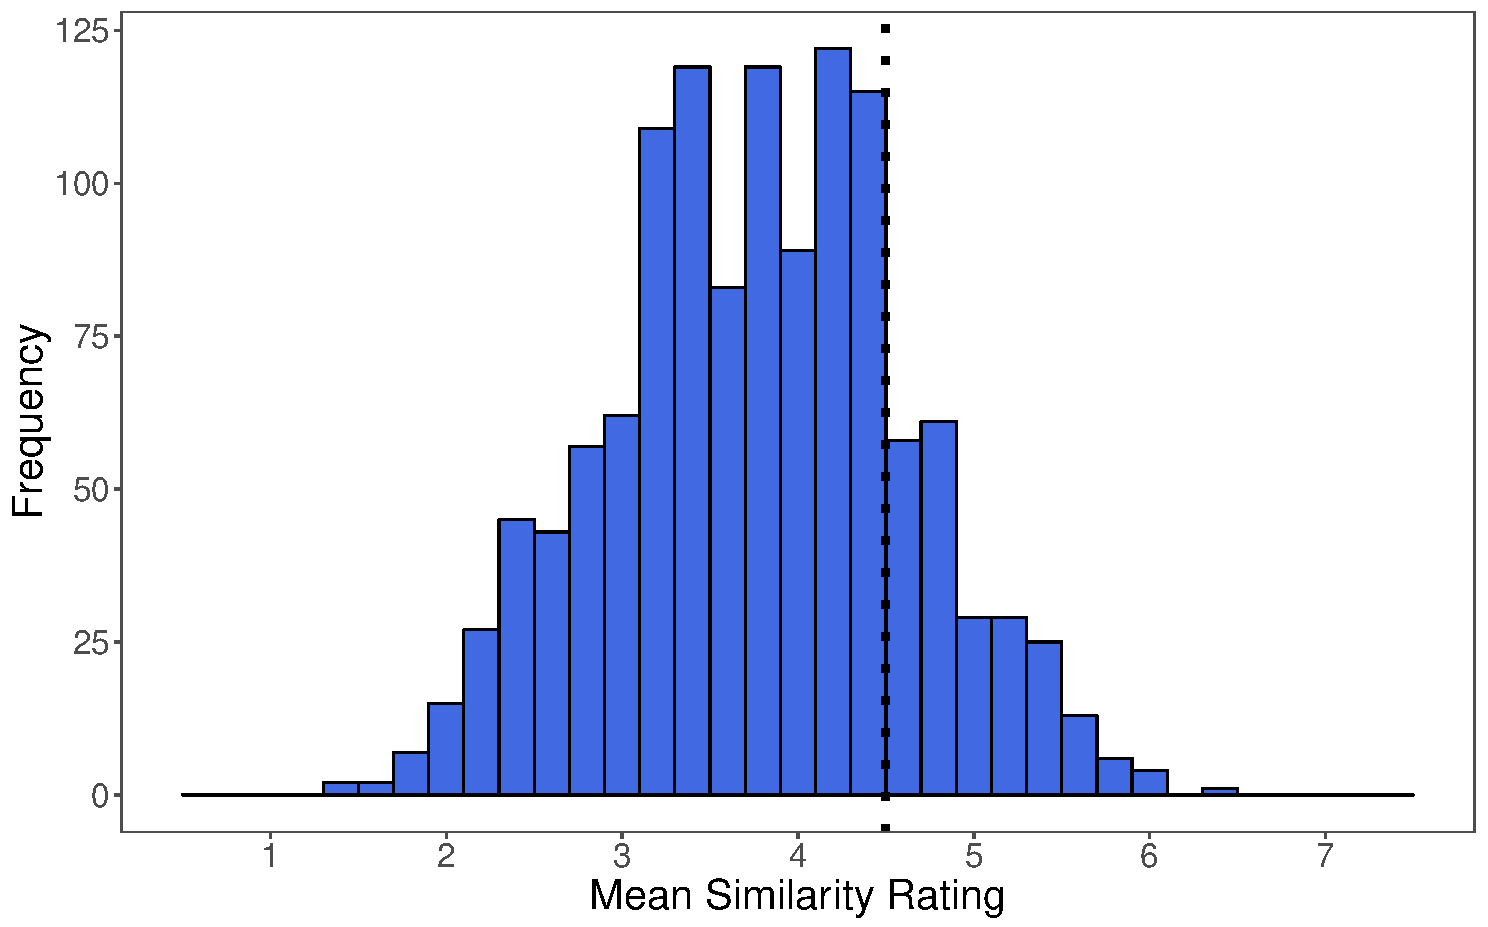
\includegraphics[width=0.9\textwidth]{figure2.pdf}
\label{fig:exp2_pilot}
\end{figure}

We decided to only use movie pairs with average ratings that are equal to or higher than 4.5, which corresponds to the upper 20\% of the similarity rating distribution (253 movie pairs). This procedure intended to ensure that our target-decoy pairs will be perceived as similar by most people.

Having created the target-decoy pairs, the next step in creating the quadruplets was to create target-competitor pairs. Since each quadruplet consists of two target-decoy pairs, we decided to pair up the 253 target-decoy pairs to create the quadruplets. To do this, we first created a target-decoy pair by target-decoy pair matrix (253x253), where each cell was the number of overlapping genre categories (obtained from IMDb) between the two movie pairs. For example, considering the comparison between target-decoy pair 1 (consisting of Movie A and Movie B) and target-decoy pair 2 (consisting of Movie C and Movie D), we summed the number of genre overlaps between movies A-C, A-D, B-C and B-D. We then selected the unique target-decoy pairs that had no genre overlap with each other. This resulted in 20,022 quadruplets, each of which is a combination of four movies (created from two movie pairs, where each movie is similar to its pair, but is distinctly different from the two movies in the other pair), created from 231 unique movies. The quadruplets used for each participant are based upon their own ratings of the 231 movies, as we describe below.


The list of movie triplets used in the experiment can be found \href{https://osf.io/fme6c/?view_only=31da4193689f4247a76af93b2f98fcef}{here}.

\subsubsection*{Experimental procedure.}

The experiment consisted of three stages: rating stage, choice stage, and a similarity rating stage. In the rating stage, we asked for participants' subjective evaluations over the 231 movies (``How do you personally rate this movie?'') on a scale from 1 (worst) to 7 (best). We also asked whether the participant had seen the movie before. The 231 movies were presented in a random order for each participant, to ensure that preference ratings are generalisable across movies from different genres. The rating stage took about 15--20 minutes.

Before the choice stage, we created a bespoke set of movie triplets for each participant using their ratings from the rating stage. First, based on each participant's preference ratings, we identified the subset of quadruplets where: (a) the target and competitor were both rated 4, both rated 5, both rated 6, or both rated 7, and (b) the two decoy movies were rated at least 3 points lower than the two target candidates. Note that we did not require the two decoys in the quadruplet to have the same rating, as it would have severely limited the number of eligible quadruplets (e.g., we allowed for quadruplets with ratings 7,7 for the two targets and 4,1 for the two decoys respectively), but we controlled for this difference in our analysis.

We then selected the subset of quadruplets where all of the movies had been seen or none of the movies had been seen, to make sure that choice behaviour will not be governed by differences in familiarity with the movies. The result was a bespoke subset of quadruplets for each participant, where the target/competitor movies had the same rating, and the decoy movies were rated worse. However, we did not want the same movie to appear twice as a target/competitor for one participant, and for this reason we used a sequential elimination technique: we first chose the quadruplet with the highest combined target-decoy similarity rating, then eliminated all quadruplets with the same target/competitor movies. We repeated these steps until we had a set a of quadruplets with unique target/competitor movies.

We only invited those participants back for whom we could create at least three unique quadruplets (corresponding to at least six attraction effect choice triplets, two per each quadruplet). In the choice stage, people were presented with the selected movie triplets in a random order, and were asked to choose the one they liked the most (see Figure \ref{fig:exp1_screenshot}).

\begin{figure}[htb!]
\centering
\caption{Choice stage.}
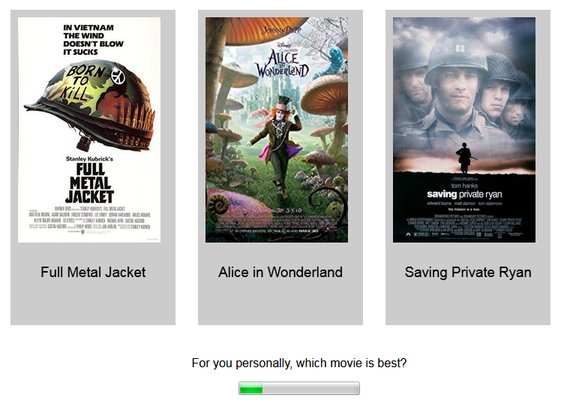
\includegraphics[width=0.8\textwidth]{rsz_exp1_choicestage.png}
\label{fig:exp1_screenshot}
\end{figure}

In the final, similarity stage, we asked participants to rate the similarity of all target-decoy and target-competitor pairs (``How similar do you think these movies are?'') on a scale from 1 (least similar) to 7 (most similar), where a ``don't know" option was also included. Information collected in this similarity rating stage was important to check that in the choice stage, participants perceived the target-decoy pairs as similar, and the target-competitor pairs as different.

We collected data in batches of 50, until we had choice data for at least a 100 participants (after all the exclusion criteria had been applied). At most, a few days have passed between the rating and choice stage. We recruited 297 English-speaking participants from Prolific Academic who were paid £8 per hour. Out of the 297 participants who completed the rating stage, we could create quadruplets for 179 participants. Out of the 179 participants who were invited back, 152 took part in the choice stage of the experiment. We did not collect any data about the demographics of our sample, as we did not expect it to affect our results.

\subsubsection*{Exclusion criteria.} \label{exclusion_ref}

To conduct a rigorous test of the attraction effect, it is crucial that people take the task seriously and reveal their true preferences. Given that individually rating 231 movies can seem somewhat mundane, we specified a set of exclusion criteria to filter those people out who did not take the rating task sufficiently seriously. These were the following. We excluded people who fell into the fastest 5\% of the reaction time distribution, the lowest 5\% of the entropy distribution and the upper and lower 5\% of the autocorrelation distribution. Entropy refers to the diversity of the ratings, while autocorrelation takes into account the temporal pattern, and measures the extent to which a response depends on previous responses. Thus, this procedure filtered out response patterns where people (a) spent an unusually short time completing the task, or (b) did not use the whole of the ratings scale, or (c) often gave the same ratings for consecutive movies, or (d) were giving ratings randomly.

These exclusion criteria were validated in a pilot study, where we collected ratings for a set of books, and included repeat trials. The participants filtered out by these three criteria were the ones who gave the least consistent ratings to repeated stimuli (correlation r $<$ .8).

When we applied these exclusion criteria to our sample of 152 people, 17 participants were filtered out, leaving a sample of 2,148 choices from 135 participants. When testing for the attraction effect, we have also removed all trials where the decoy was chosen.


\subsection*{Results}

The median number of choice trials per participant was 16 (range 6--54), and 84\% of participants were presented with at least 8 choice trials. The decoy was only chosen in 4.3\% of the trials. In addition, 72\% of participants never chose the decoy, and only 2\% chose it in more than 25\% of the trials. This indicates that participants were able to identify the dominated decoy in the choice stage. 

In the attraction effect, the decoy increases the choice share of the target at the expense of the competitor. Figure \ref{fig:exp2_res} shows the proportions of trials where the target was chosen instead of the competitor (excluding all trials where the decoy was chosen, as specified in our preregistration). Each point corresponds to a participant. The mean proportion of trials where the target was chosen is M=.50, 95\% CI [.49--.51], which demonstrates that participants were almost perfectly indifferent between the target and the competitor, and that the attraction effect is virtually zero. A one-sample $t$-test shows that the proportion of trials where the target was chosen is not significantly higher than .5, $t(134)=-.44$, $p=.669$. 

\begin{figure}[htb!]
\centering
		\caption{The proportion of trials where the target was chosen instead of the competitor. Each dot is a participant. Dots are jittered slightly. The red dot and error bars show the bootstrapped mean and 95\% CI under stratified sampling (by participant).}
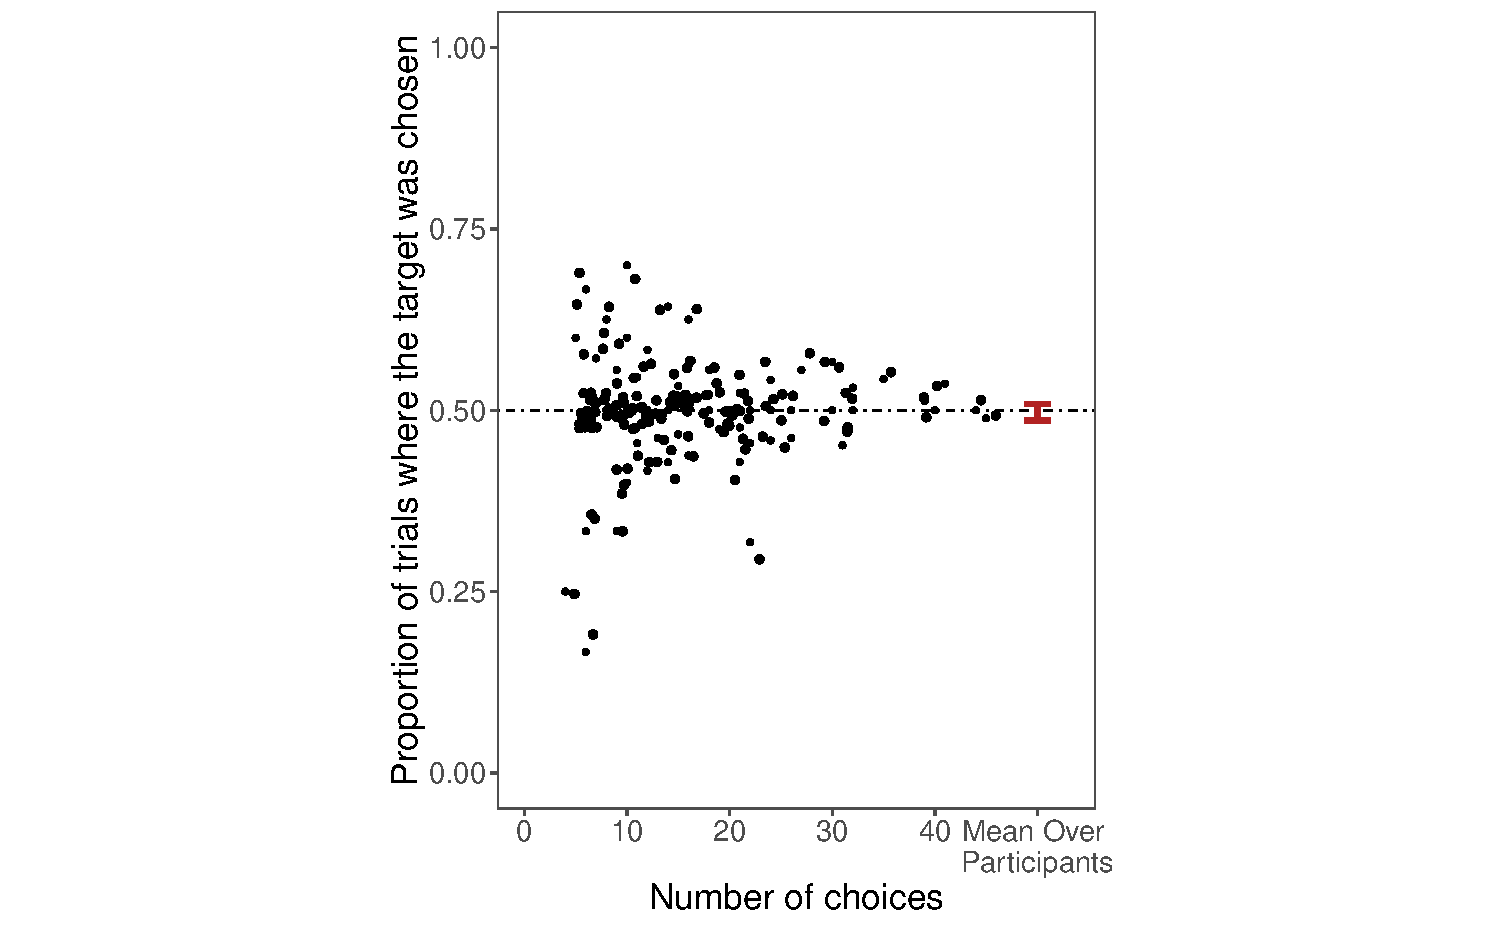
\includegraphics[width=0.9\textwidth]{figure4.pdf}
\label{fig:exp2_res}
\end{figure}

We created the choice triplets carefully so that the target-decoy pairs were perceived as similar, and the target-competitor pairs were perceived as different. To ensure that our participants indeed perceived the triplets this way, we compared the distribution of the target-decoy and target-competitor similarity ratings. As Figure \ref{fig:exp2_similarityratings} shows, the overwhelming majority of target-competitor pairs were perceived as not similar, while the majority of target-decoy pairs were perceived as similar, exactly as we intended.

\begin{figure}[htb!]
\centering
		\caption{Distribution of the target-competitor and target-decoy similarity ratings.}
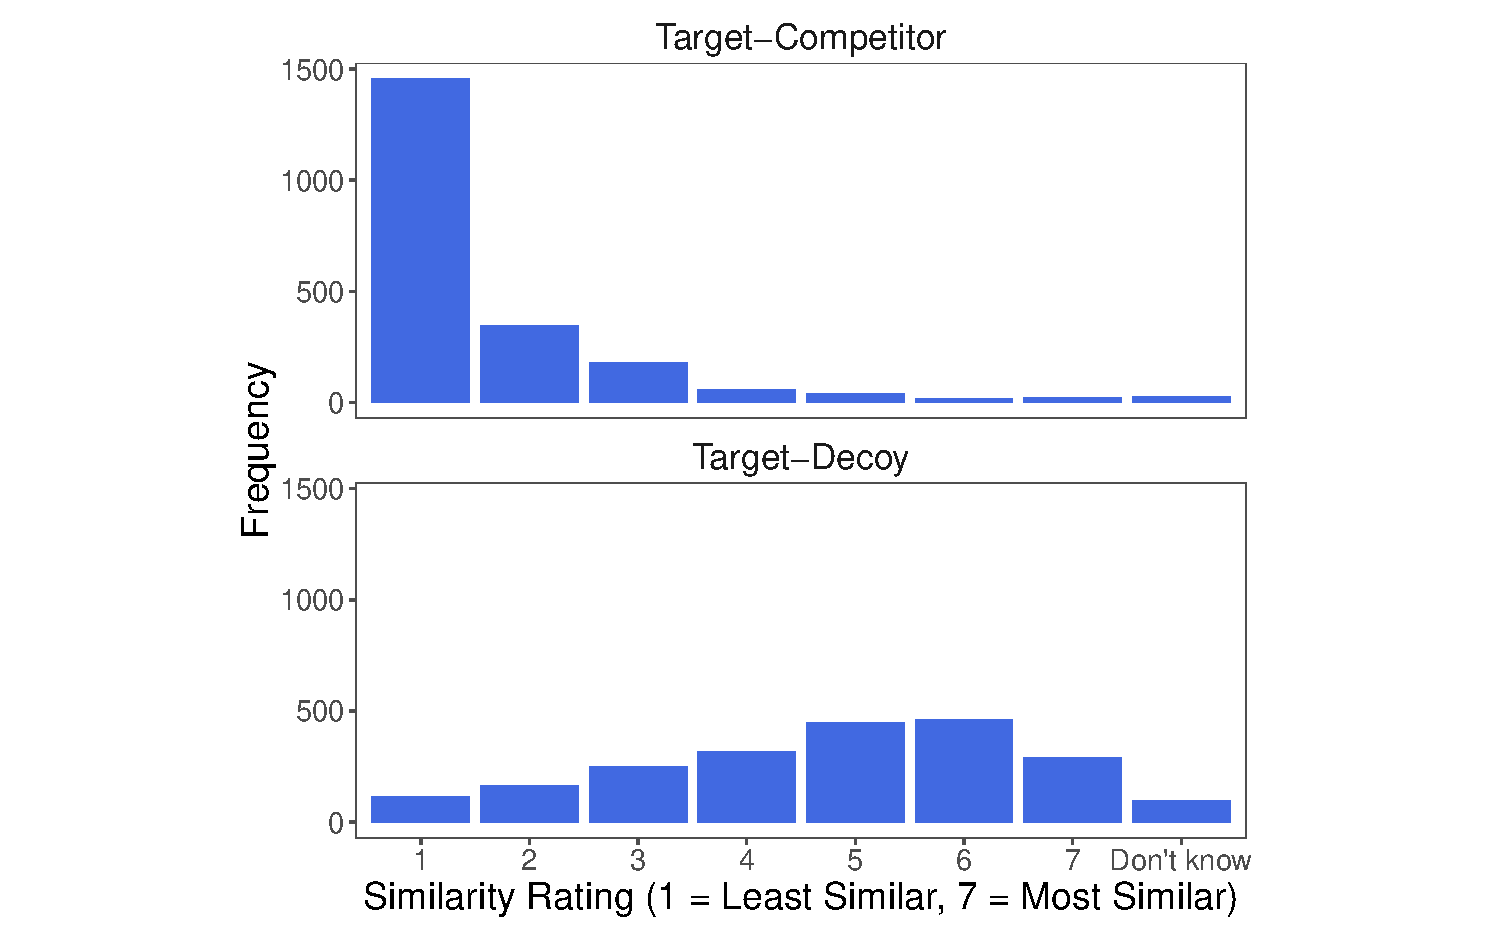
\includegraphics[width=0.8\textwidth]{Figure5.pdf}
\label{fig:exp2_similarityratings}
\end{figure}


To account for subject-specific variability, we also estimated the likelihood of choosing the target with an intercept-only mixed effects logistic regression with by-subjects intercepts (see Model 1 in Table \ref{latentattr_exp2reg}). The odds of 1 for choosing the target over the competitor reflect equal preference for the target and competitor, and corresponds to the choice proportion of .5 in Figure \ref{fig:exp2_res}. Using Model 1, we calculate that the overall probability of choosing the target is .50, 95\% CI [.48--.52], the same what we see in the mean over subject proportions from Figure \ref{fig:exp2_res}.


\begin{table*}[htb!]
\centering
  \begin{threeparttable}
    \caption{Odds ratios and 95\% CIs from two mixed-effects logistic models fit by maximum likelihood with subject-specific intercepts.}
  \label{latentattr_exp2reg}
\begin{tabular}{@{\extracolsep{5pt}}lcc}
\\[-1.8ex]\hline
\hline \\[-1.8ex]
 & \multicolumn{2}{c}{\textit{Dependent variable:}} \\
\cline{2-3}
\\[-1.8ex] & \multicolumn{2}{c}{Target chosen} \\
 & Model 1 & Model 2 \\
\hline \\[-1.8ex]
 Intercept & 1.001 (0.918, 1.091) & 0.987 (0.802, 1.214) \\
  Seen all &  & 1.046 (0.690, 1.587) \\
  TC similarity rating &  & 0.981 (0.895, 1.075) \\
  TD similarity rating &  & 0.960 (0.877, 1.050) \\
  TD rating difference &  & 0.944 (0.863, 1.032) \\
 \hline \\[-1.8ex]
Observations & 2,055 & 1,953 \\
Log Likelihood & $-$1,424.417 & $-$1,352.312 \\
Akaike Inf. Crit. & 2,852.834 & 2,716.624 \\
Bayesian Inf. Crit. & 2,864.090 & 2,750.087 \\
\hline
\hline \\[-1.8ex]
%\textit{Note:}  & \multicolumn{2}{r}{$^{*}$p$<$0.1; $^{**}$p$<$0.05; $^{***}$p$<$0.01} \\
\end{tabular}
    \begin{tablenotes}
      \small
      \item Notes: $^{*}$p$<$0.05; ratings have been scaled; Seen all is coded 0.5 (Yes) and -0.5 (No); T - Target, C - Competitor, D - Decoy
    \end{tablenotes}
  \end{threeparttable}
\end{table*}

We also ran a mixed effects logistic regression with by-subjects intercepts to investigate how participants' target-decoy and target-competitor similarity ratings, familiarity with the movies, and target-decoy preference rating difference affect the likelihood of choosing the target (see Model 2 in Table \ref{latentattr_exp2reg}). The sample size is slightly smaller because people giving ``Don't Know'' ratings were not included. None of the ratings modulate the strength of the attraction effect. The overall probability of choosing the target is .50, 95\% CI [.44--.55], with a slightly wider confidence interval. The conclusion from the two models and the simple mean over proportions is the same: we estimate a precisely zero attraction effect.

\subsubsection*{Further analyses}


Our experimental design ensured that for each bespoke A B movie pair, participants were presented with both A, B, A' and B, A, B' triplets. Faced with two subsequent choices involving two equally highly rated A--B movie pairs and two different, but undesirable decoys, it is possible that the first choice is  ``sticky'', and will be repeated. If this is the case, then we can expect that the target and the competitor will be chosen exactly half of the time, resulting in a perfectly zero attraction effect. 

Indeed, participants were overwhelmingly likely to stick with their first choice, as they only switched between A and B in 8.5\% of cases (out of the 990 bespoke A--B pairs where the decoy was not chosen on either of the first or second trial). Out of these 84 cases when participants switched, 48 times they have chosen the target both times. This means that we found no evidence that the proportion of switches towards the attraction effect (i.e., choosing the target on both occasions as opposed to always choosing the competitor) was significantly higher than 0.5, ${\chi}^2(1, N = 84)=1.44$, $p=.115$, 95\% CI [.46--.68].

Even though participants tended to stick with their first choice, the attraction effect might still be evident on the first choice for each bespoke A--B pair, and if this the case we can also expect a ``reverse'' attraction effect (higher likelihood of choosing the competitor) on the second choice. After excluding individual trials where the decoy was chosen, we found no evidence that the proportion of trials where the target was chosen was different from .5 on the first, $t(134)=-.039$, $p=.969$, 95\% CI [.46--.52], or second choice, $t(134)= .015$, $p=.988$, 95\% CI [.48--.54].

Our experimental design relies on the assumption that participants should be indifferent between equally highly rated movies from different genres. However, if the cognitive processes underlying the evaluation and choice stages are different, then discrepancies between ratings and choices might arise. For example, it is possible that the rating reflects preference for the movie \textit{within} its genre category, but the overall choice between two movies with different genres is driven by overall genre preferences.


To address this concern, we first tested whether overall genre preferences have an influence on choices over and above the information reflected in individual movie ratings, by adding the difference between the target–competitor genre ratings for each participant to our regression models described in Table \ref{latentattr_exp2reg} (Model 1 and 2), assuming that average genre ratings serve as a suitable proxy for overall genre preferences. The results in Table \ref{latentattr_exp3reg} in the Appendix show that while overall genre preferences do not change our previous estimates when added to an intercept-only regression (Model 3), the probability of choosing the target slightly increases when all other explanatory variables are also included in the regression (Model 4). Specifically, one standard deviation increase in the difference of the average target-competitor rating (corresponding to a 0.9 unit increase in average ratings on the original rating scale) increases the odds of choosing the target by about 10\%.  
 

Second, to determine whether overall genre preferences influence the strength of the attraction effect, we tested the attraction effect using the subset of trials where overall genre preferences were roughly equal. Using, a one-sample $t$-test on a subset of trials where absolute difference between the average target and competitor genre ratings was less than 0.25 (about 23\% of all trials), we found no evidence that the proportion of trials where the target was chosen was higher than .5, $t(98)=-.142$, $p=.556$, 95\% CI [.46--.55].
  
Overall, while the results indicate that overall genre preferences slightly influenced choices between the target and competitor, we found no evidence that this had any effect on the strength of the attraction effect.

The decoy was chosen very rarely, in less than 5\% of trials. Previously, it had been shown that a decoy that is placed too far from the target can result in a reverse attraction effect (repulsion effect; \citeNP{Spektor2018}). On a 1-7 preference rating scale, we allowed for a minimum distance of 3 and a maximum of 6 between the target and decoy. While we have not find any evidence that the target-decoy rating difference influenced the strength of the attraction effect (see Model 2 in Table \ref{latentattr_exp2reg}), a non-linear association between target-decoy preference and the attraction effect might still exist. To examine this possibility whilst controlling for the perceived similarity of the target-decoy pair, we ran a logistic regression model to predict the probability of choosing the target, with target-decoy rating difference and their perceived similarity as explanatory variables. To test for a potential non-monotonic relationship, we estimated a separate coefficient for each level of the explanatory variables. Figure \ref{fig:exp2_res_app1}  in the Appendix shows the predicted probabilities from this analysis for each combination of target-decoy rating difference and similarity. We found no evidence for the hypothesis that the strength of the attraction effect varies by target-decoy rating difference and similarity rating.

While not part of our pre-registered analysis plan, it is possible that the strength of the attraction effect is influenced by the overall preference for the target and competitor (this is at least 4 and at most 7 in our experiment). To explore this possibility, we calculated the proportion of trials where the target was chosen for each level of target-competitor preference rating. Figure \ref{fig:exp2_res_app2} in the Appendix shows these proportions, suggesting that target-competitor preference ratings had no effect on the strength of the attraction effect. 


\section*{General Discussion}

We tested for the attraction effect in a choice task with naturalistic choice options. We found that the presence of the decoy in the choice set did not alter preferences over the target and the competitor, as participants remained perfectly indifferent between the target and competitor. Our experimental design was carefully developed to test the attraction effect with naturalistic stimuli whilst avoiding the five critical conditions set out by \citeA{Huber2014}.

First, we created bespoke choice triplets with the equal preference ratings for the target and competitor, with the aim to ensure participants' indifference between the target and the competitor, maximising the probability that choices will be constructed on the spot (rather than through relying on strong prior preferences), and that an attraction effect will occur. While we found some evidence that overall genre ratings have influenced choices between the target and competitor over and above their preference ratings, this effect was small (also illustrated by the fact that in only 53\% of trials participants chose the movie with the higher average genre rating). Most importantly, the strength of the attraction effect was not influenced by overall genre preferences. 

Second, we have strong evidence that the dominance relationship was perceived in our experiment. The target-decoy similarity ratings confirmed that our careful target-decoy selection process resulted in movie pairs that were perceived as similar. In addition, our choice set construction criteria ensured that the decoy was always rated at least 3 units lower than the target (and the competitor). Consequently, the decoy was only chosen in 4.3\% of the trials, which clearly shows that participants were able to spot and avoid the dominated option. These choice patterns strongly suggest that participants expressed their true preferences, despite the experimental design not being incentive-compatible.

Third, by creating bespoke choice triplets based on the ratings, we avoided individual heterogeneity in preferences as a potential confound. In addition, we ensured that the decoy is not too desirable in comparison to the target. We also used a strict exclusion criteria to filter out participants who did not take the task sufficiently seriously, and with an average of 16 choice trials per participant, we avoided participant fatigue.

Finally, in our analysis, we controlled for familiarity with the choice options, perceived similarity of the target-decoy and target-competitor pair, and preference difference between the target and the decoy, but we found that none of these modulated or revealed an attraction effect. The fact that the preference difference between the target and the decoy did not affect the strength of the attraction effect suggests that our results did not arise from a potentially undesirable decoy. 


In conclusion, our results are in line with that of \citeA{Frederick2014}, and provide strong evidence that the attraction effect does not extend to choice between naturalistic options. While we did not aim to investigate the exact reason behind why the attraction effect is robust in choices involving numerical attribute dimensions but is absent from choices involving naturalistic options, we hypothesize that the separability of the attribute dimensions is an important factor. More specifically, while there is strong evidence that attribute-wise comparison strategies are key to the attraction effect in numerical or perceptual choices, such comparison strategies are less likely to occur with complex, naturalistic objects. Future research could test this hypothesis by exploring how the comparison process and the strength of the attraction effect varies with different representations of the same choice options (separate attributes versus naturalistic representation), extending \citeauthor{Frederick2014}'s investigation of numerical versus visual presentation of the same stimuli. Results from such experiments could provide us with important insights about the boundary conditions of the attraction effect, and the cognitive process underlying this choice bias.




\bibliographystyle{apacite}


%\theendnotes


\newpage

\bibliography{refs_update}

\clearpage
\begin{appendices}

\renewcommand{\thetable}{A\arabic{table}}
\renewcommand{\thefigure}{A\arabic{figure}}
\setcounter{table}{0}
\setcounter{figure}{0}

%\begin{table*}[htb!]
%\centering
%  \begin{threeparttable}
%    \caption{Odds ratios and 95\% CIs from two mixed-effects logistic models fit by maximum likelihood with subject-specific intercepts.}
%  \label{latentattr_exp3reg}
%\begin{tabular}{@{\extracolsep{5pt}}lcc} 
%\\[-1.8ex]\hline 
%\hline \\[-1.8ex] 
% & \multicolumn{2}{c}{\textit{Dependent variable:}} \\ 
%\cline{2-3} 
%\\[-1.8ex] & \multicolumn{2}{c}{Target chosen} \\ 
% & Model 3 & Model 4 \\ 
%\hline \\[-1.8ex] 
%Intercept & 0.989 (0.803, 1.217) & 0.991 (0.805, 1.221) \\
% Seen all & 1.042 (0.687, 1.581) & 1.037 (0.684, 1.575) \\ 
%  TC similarity rating& 0.980 (0.895, 1.074) & 0.981 (0.895, 1.075) \\ 
% TD similarity rating & 0.960 (0.877, 1.050) & 0.960 (0.877, 1.050) \\ 
%  TD rating difference & 0.947 (0.866, 1.036) & 0.947 (0.865, 1.036) \\ 
%  TC genre rating difference & 1.101$^{*}$ (1.007, 1.204) & 1.101$^{*}$ (1.007, 1.204) \\ 
%  Preferred genre chosen &  & 0.969 (0.810, 1.158) \\  
% \hline \\[-1.8ex] 
%Observations & 1,953 & 1,953 \\ 
%Log Likelihood & $-$1,350.093 & $-$1,350.032 \\ 
%Akaike Inf. Crit. & 2,714.186 & 2,716.064 \\ 
%Bayesian Inf. Crit. & 2,753.226 & 2,760.681 \\ 
%\hline 
%\hline \\[-1.8ex] 
%%\textit{Note:}  & \multicolumn{2}{r}{$^{*}$p$<$0.1; $^{**}$p$<$0.05; $^{***}$p$<$0.01} \\ 
%\end{tabular} 
%    \begin{tablenotes}
%      \small
%      \item Notes: $^{*}$p$<$0.05; ratings, and rating differences have been scaled; Seen all and Preferred genre chosen is coded 0.5 (Yes) and -0.5 (No); T - Target, C - Competitor, D - Decoy
%    \end{tablenotes}
%  \end{threeparttable}
%\end{table*}


\begin{table*}[htb!]
\centering
  \begin{threeparttable}
    \caption{Odds ratios and 95\% CIs from two mixed-effects logistic models fit by maximum likelihood with subject-specific intercepts.}
  \label{latentattr_exp3reg}
\begin{tabular}{@{\extracolsep{5pt}}lcc} 
\\[-1.8ex]\hline 
\hline \\[-1.8ex] 
 & \multicolumn{2}{c}{\textit{Dependent variable:}} \\ 
\cline{2-3} 
\\[-1.8ex] & \multicolumn{2}{c}{Target chosen} \\ 
 & Model 3 & Model 4 \\ 
\hline \\[-1.8ex] 
Intercept & 1.001 (0.918, 1.091) & 0.989 (0.803, 1.217) \\ 
 Genre rating difference & 1.080 (0.990, 1.178) & 1.101$^{*}$ (1.007, 1.204) \\  
 Seen all &  & 1.042 (0.687, 1.581) \\ 
  TC similarity rating &  & 0.980 (0.895, 1.074) \\ 
  TD similarity rating &  & 0.960 (0.877, 1.050) \\ 
  TD rating difference &  & 0.947 (0.866, 1.036) \\ 
   \hline \\[-1.8ex]
Observations & 2,055 & 1,953 \\ 
Log Likelihood & $-$1,422.902 & $-$1,350.093 \\ 
Akaike Inf. Crit. & 2,851.803 & 2,714.186 \\ 
Bayesian Inf. Crit. & 2,868.687 & 2,753.226 \\ 
\hline 
\hline \\[-1.8ex] 
%\textit{Note:}  & \multicolumn{2}{r}{$^{*}$p$<$0.1; $^{**}$p$<$0.05; $^{***}$p$<$0.01} \\ 
\end{tabular} 
    \begin{tablenotes}
      \small
      \item Notes: $^{*}$p$<$0.05; ratings, and rating differences have been scaled; Seen all is coded 0.5 (Yes) and -0.5 (No); T - Target, C - Competitor, D - Decoy
    \end{tablenotes}
  \end{threeparttable}
\end{table*}


\begin{figure}[htb!]
\centering
		\caption{The predicted proportion of trials where the target was chosen instead of the competitor, by target decoy rating difference and similarity rating. The dot and error bars show model predictions and 95\% CIs from a logistic regression with target-decoy similarity rating and rating difference as explanatory variables.}
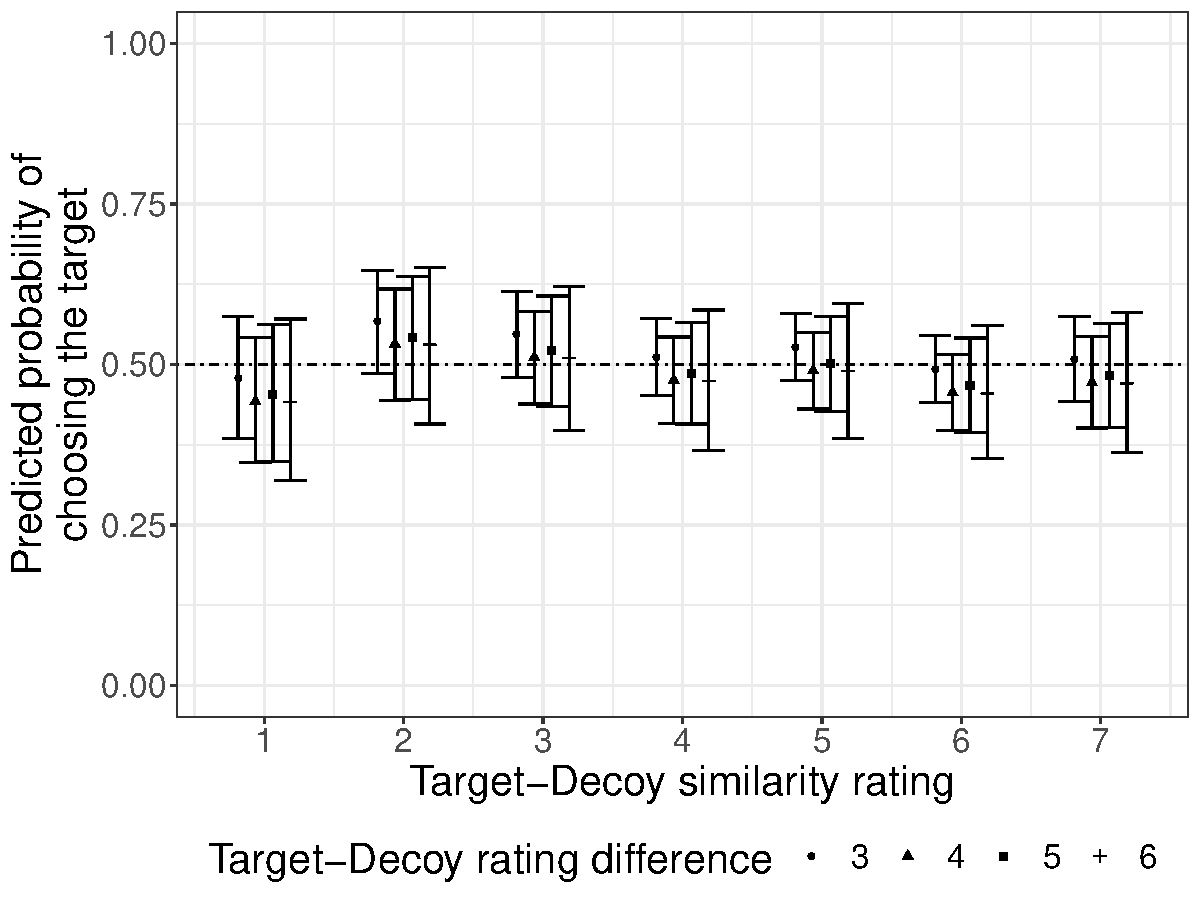
\includegraphics[width=0.9\textwidth]{figure6.pdf}
\label{fig:exp2_res_app1}
\end{figure}



\begin{figure}[htb!]
\centering
		\caption{The proportion of trials where the target was chosen instead of the competitor by target-competitor rating. The dots and error bars show the bootstrapped mean and 95\% CI under stratified sampling (by participant).}
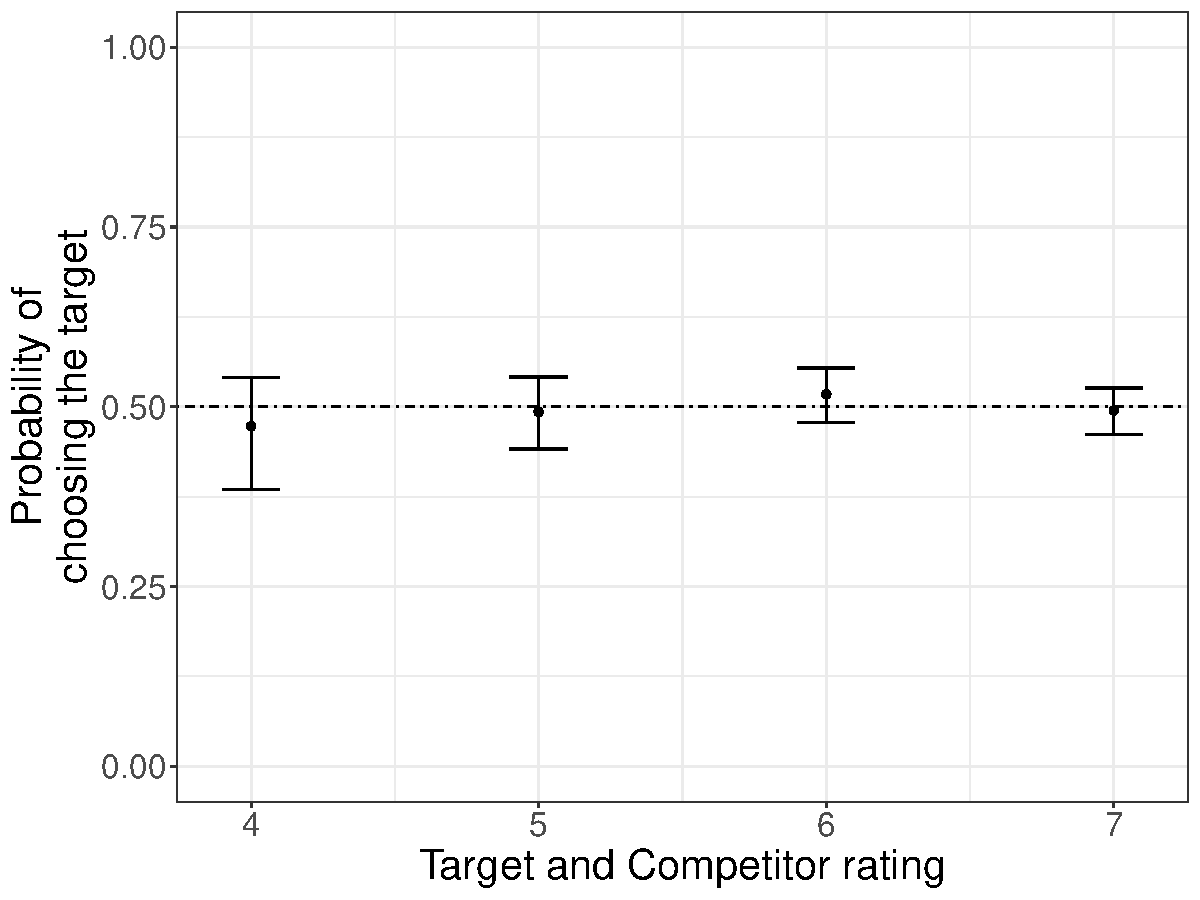
\includegraphics[width=0.9\textwidth]{figure7.pdf}
\label{fig:exp2_res_app2}
\end{figure}

\end{appendices}

\end{document}
